%\newpage
%\section{Appendix}
\section{Proof of Theorem~\ref{thm:general_alpha}}
\label{sec:proof-performance_guarantee}

We first prove Theorem~\ref{thm:general_alpha}, then we specify the value of $\alpha$ to obtain Theorem~\ref{thm:thm_performance_guarantee} as a specific case of Theorem~\ref{thm:general_alpha}. The proof of Theorem~\ref{thm:general_alpha} is divided into two parts. 

In part 1, we prove that if \underline{$l(\theta;G) < \beta + \triangle$ (even if $l(\theta;G) \geq \beta$)}, for any $\alpha \in (0, 2/L)$ Meta-GNN with one-step finetuning outputs \underline{a feasible solution $X$ of good quality} $f(X;G)\leq l(\theta;G)-\triangle$. Here, $\triangle = \|\nabla_{\theta} l(\theta;G)\| \epsilon + \frac{1}{2L\alpha^2 - 4\alpha}\epsilon^2$ if $\epsilon < \alpha \|\nabla_{\theta} l(\theta;G)\|$ or $\triangle = (\alpha - \frac{L\alpha^2}{2})\|\nabla_{\theta}l(\theta;G)\|^2$ o.w..

In part 2, we prove that once \proj achieves the loss value $l(\theta';G)$ after the one-step finetuning, the rounding process would output a feasible $X$ whose objective satisfies $f(X;G)\leq l(\theta';G)$. 

\textbf{Part 1:}We could get 
\begin{equation}
\begin{aligned}
l(\theta';G) 
& \stackrel{(a)}{\leq} l(\theta;G) + \nabla_{\theta}l(\theta;G)(\theta'-\theta) + \frac{1}{2}L \| \theta' - \theta\|_2^2\\
& \stackrel{(b)}{=} l(\theta;G) + \frac{1}{2}L\|\theta' - \theta\|_2^2 - \alpha \|\nabla_{\theta} l(\theta;G)\|_2^2 \\
&  = l(\theta;G)+ (\frac{L\alpha^2}{2} - \alpha) \|\nabla_{\theta} l(\theta;G)\|_2^2,
\end{aligned}
\end{equation}
where (a) is due to the local L-smoothness of $l(\cdot;G)$, (b) is due to the definition of one-step finetuning $\theta' = \theta - \alpha \nabla_{\theta}l(\theta;G)$.

If $\epsilon < \alpha \|\nabla_{\theta}l(\theta;G)\|$:

\qquad Let $\triangle = \|\nabla_{\theta} l(\theta;G)\| \epsilon + \frac{1}{2L\alpha^2 - 4\alpha}\epsilon^2$, we have:
\begin{equation}
\begin{aligned}
\min_{\epsilon} - \triangle & = \min_{\epsilon} -\frac{1}{2L\alpha^2 - 4\alpha} \epsilon^2 - \|\nabla_{\theta}l(\theta;G)\|\epsilon  = (\frac{L\alpha^2}{2}-\alpha)\|\nabla_{\theta}l(\theta;G)\|^2,
\end{aligned}
\end{equation}

\qquad thus
\begin{equation}
\begin{aligned}
    l(\theta';G) &\leq l(\theta;G) - \triangle.
\end{aligned}
\end{equation}

If $\epsilon \geq \alpha \|\nabla_{\theta}l(\theta;G)\|$:

\qquad Let $\triangle = (\alpha - \frac{L\alpha^2}{2})\|\nabla_{\theta}l(\theta;G)\|^2$, we would directly have:
\begin{equation}
\begin{aligned}
    l(\theta';G) &\leq l(\theta;G) - \triangle.
\end{aligned}
\end{equation}
By this, we finish the first part of the proof for Theorem~\ref{thm:general_alpha}. 

\textbf{Part 2:} The proof in this part follows the rounding analysis in ~\cite{wang2022unsupervised}. Consider the rounding procedure from continuous space $\bar{X} = \mathcal{A}_{\theta}(G), \bar{X} \in [0,1]^n$ into the discrete feasible solution $X \in \{0,1\}^n$. Let $\bar{X}_i, X_i, i = \{0,1,...,n\}$ denote their entries. W.l.o.g, suppose the rounding order is from $1$ to $n$ and we have finished the rounding before the $t$-th node, we now analyze the rounding of $t$-th node:
\begin{equation}
\begin{aligned}
    %& l(\theta';G) \\
    & f_r([X_1,...,X_{t-1},\bar{X}_t,\bar{X}_{t+1},...,\bar{X}_n];G) + \beta g_r([X_1,...,X_{t-1},\bar{X}_t,\bar{X}_{t+1},...,\bar{X}_n];G) \\
      \stackrel{(d)}{\geq} & \bar{X}_t ( f_r([X_1,...,X_{t-1},1,\bar{X}_{t+1},...\bar{X}_n];G) + \beta g_r([X_1,...,X_{t-1},1,\bar{X}_{t+1},...,\bar{X}_n];G)) \\
    & + (1-\bar{X}_t) ( f_r([X_1,...,X_{t-1},0,\bar{X}_{t+1},...,\bar{X}_n];G) + \beta g_r([X_1,...,X_{t-1},0,\bar{X}_{t+1},...,\bar{X}_n];G)) \\
    \geq & \bar{X}_t ( \min_{j_t=\{0,1\}}f_r([X_1,...,X_{t-1},j_t,\bar{X}_{t+1},...,\bar{X}_n];G) + \beta g_r([X_1,...,X_{t-1},j_t,\bar{X}_{t+1},...,\bar{X}_n];G)) \\
    & + (1-\bar{X}_t) (\min_{j_t=\{0,1\}} f_r([X_1,...,X_{t-1},j_t,\bar{X}_{t+1},...,\bar{X}_n];G) \\
    &+ \beta g_r([X_1,...,X_{t-1},j_t,\bar{X}_{t+1},...,\bar{X}_n];G)) \\
     \stackrel{(e)}{=} & f_r([X_1,...,X_{t-1},X_t,\bar{X}_t,...,\bar{X}_n];G) + \beta g_r([X_1,...,X_{t-1},X_t,\bar{X}_t,...,\bar{X}_n];G) \\
\end{aligned}
\end{equation}
where (d) is due to $l_r(\theta;G)$'s entry-wise concavity w.r.t $\bar{X}$ and Jensen's inequality, (e) is due to $X_t = \arg\min_{j=0,1} f_r(X_1,...,X_{t-1},t,\bar{X}_{t+1},...,\bar{X}_n)+\beta g_r(X_1,...,X_{t-1},t,\bar{X}_{t+1},...,\bar{X}_n)$ (the definition of our rounding process). The loss value is monotonically non-increasing through the whole rounding process according to the equation above, thus we could get:
\begin{equation}
    l(\theta') \geq f(X;G) + \beta g(X;G)
\end{equation}
By this, we finish the proof of the second part.

\subsection{A Specific Case}
Note that in the first part of the proof above, if we specify the value of $\alpha$ as $\frac{1}{L}$ in equation (6), we could have:
\begin{equation}
    l(\theta';G) \leq l(\theta;G) -\frac{\|\nabla_{\theta}l(\theta;G)\|_2^2}{2L} 
\end{equation}
If $\epsilon< \frac{1}{L}\|\nabla_{\theta} l(\theta;G)\|$:

\qquad Let $\triangle = \|\nabla_{\theta}l(\theta;G)\| \epsilon - \frac{L}{2}\epsilon^2$, we have: 

\begin{equation}
\begin{aligned}
\min_{\epsilon} - \triangle & = \min_{\epsilon} \frac{L}{2} \epsilon^2 - \|\nabla_{\theta}l(\theta;G)\|\epsilon  = -\frac{\|\nabla_{\theta}l(\theta;G)\|^2}{2L},
\end{aligned}
\end{equation}
\qquad thus
\begin{equation}
\begin{aligned}
    l(\theta';G) &\leq l(\theta;G) - \triangle.
\end{aligned}
\end{equation}


If $\epsilon \geq \frac{1}{L}\|\nabla_{\theta} l(\theta;G)\|$:

\qquad Let $\triangle = \frac{1}{2L}\|\nabla_{\theta}l(\theta;G)\|^2$, we would directly have:
\begin{equation}
\begin{aligned}
    l(\theta';G) &\leq l(\theta;G) - \triangle.
\end{aligned}
\end{equation}
By this, we obtain Theorem~\ref{thm:thm_performance_guarantee}, a specific case of Theorem~\ref{thm:general_alpha} as follows:

\begin{theorem}[A Specific case of Theorem~\ref{thm:general_alpha}]
\label{thm:thm_performance_guarantee}
Suppose the relaxations $f_r$ and $g_r$ are entry-wise concave as required in \citep{wang2022unsupervised}. Let $\theta$ denote the learned parameter after training.  Given a test instance $G$, suppose locally $l(\cdot;G)$ is $L$-smooth at $\theta$, i.e., $\|\nabla_{\theta'} l(\theta';G) - \nabla_{\theta} l(\theta;G)\|\leq L\|\theta' - \theta\|$ for all $\theta'$ that satisfies $\|\theta' - \theta\|\leq \epsilon$. Then, if \underline{$l(\theta;G) < \beta + \triangle$ (even if $l(\theta;G) \geq \beta$)}, there exists $\alpha$ such that Meta-GNN with one-step finetuning outputs \underline{a feasible solution $X$ of good quality} $f(X;G)\leq l(\theta;G)-\triangle$. Here, $\triangle = \|\nabla_{\theta} l(\theta;G)\|\epsilon - \frac{L}{2}\epsilon^2$ if $\epsilon< \frac{1}{L}\|\nabla_{\theta} l(\theta;G)\|$ or $\triangle=\frac{1}{2L}\|\nabla_{\theta} l(\theta;G)\|^2$ o.w..
\end{theorem}


\vspace{0.2cm}


\iffalse
\subsection{Theorem ~\ref{thm:thm_performance_guarantee}: A More General Case}
In Theorem~\ref{thm:thm_performance_guarantee}, we proved the performance guarantee of \proj when the inner learning rate $\alpha$ is set as $1/L$ as the best case. Here we extend the value of $\alpha$ into general cases and show that our theorem still holds.

\begin{theorem}[General case for Theorem~\ref{thm:thm_performance_guarantee}]
\label{thm:general_alpha2}
Suppose the relaxations $f_r$ and $g_r$ are entry-wise concave as required in \citep{wang2022unsupervised}. Let $\theta$ denote the learned parameter after training.  Given a test instance $G$, suppose locally $l(\cdot;G)$ is $L$-smooth at $\theta$, i.e., $\|\nabla_{\theta'} l(\theta';G) - \nabla_{\theta} l(\theta;G)\|\leq L\|\theta' - \theta\|$ for all $\theta'$ that satisfies $\|\theta' - \theta\|\leq \epsilon$. Then, if \underline{$l(\theta;G) < \beta + \triangle$ (even if $l(\theta;G) \geq \beta$)}, for any $\alpha \in (0, 2/L)$ Meta-GNN with one-step finetuning outputs \underline{a feasible solution $X$ of good quality} $f(X;G)\leq l(\theta;G)-\triangle$. Here, $\triangle = \|\nabla_{\theta} l(\theta;G)\| \epsilon + \frac{1}{2L\alpha^2 - 4\alpha}\epsilon^2$ if $\epsilon < \alpha \|\nabla_{\theta} l(\theta;G)\|$ or $\triangle = (\alpha - \frac{L\alpha^2}{2})\|\nabla_{\theta}l(\theta;G)\|^2$ o.w..
\end{theorem}

\textbf{Proof of Theorem~\ref{thm:general_alpha}:} We divide our proof into two parts. In part 1, we prove that . In part 2, we need to prove that once \proj achieves the loss value $l'(\theta;G)$ after the one-step finetuning, the rounding process would output a feasible solution such that $f(X;G)\leq l(\theta';G)$. The proof of part 2 is exactly the same as that for Theorem~\ref{thm:thm_performance_guarantee}, therefore we only provided the details of part 1 as follows:
By Taylor Expansion, we could get 
\begin{equation}
\begin{aligned}
l(\theta';G) 
& \stackrel{(a)}{\leq} l(\theta;G) + \nabla_{\theta}l(\theta;G)(\theta'-\theta) + \frac{1}{2}L \| \theta' - \theta\|_2^2\\
& \stackrel{(b)}{=} l(\theta;G) + \frac{1}{2}L\|\theta' - \theta\|_2^2 - \alpha \|\nabla_{\theta} l(\theta;G)\|_2^2 \\
&  = l(\theta;G)+ (\frac{L\alpha^2}{2} - \alpha) \|\nabla_{\theta} l(\theta;G)\|_2^2,
\end{aligned}
\end{equation}
where (a) is due to the local L-smoothness of $l(\cdot;G)$, (b) is due to the definition of one-step finetuning $\theta' = \theta - \alpha \nabla_{\theta}l(\theta;G)$.

If $\epsilon < \alpha \|\nabla_{\theta}l(\theta;G)\|$:

\qquad Let $\triangle = \|\nabla_{\theta} l(\theta;G)\| \epsilon + \frac{1}{2L\alpha^2 - 4\alpha}\epsilon^2$, we have:
\begin{equation}
\begin{aligned}
\min_{\epsilon} - \triangle & = \min_{\epsilon} -\frac{1}{2L\alpha^2 - 4\alpha} \epsilon^2 - \|\nabla_{\theta}l(\theta;G)\|\epsilon  = (\frac{L\alpha^2}{2}-\alpha)\|\nabla_{\theta}l(\theta;G)\|^2,
\end{aligned}
\end{equation}

\qquad thus
\begin{equation}
\begin{aligned}
    l(\theta';G) &\leq l(\theta;G) - \triangle.
\end{aligned}
\end{equation}

If $\epsilon \geq \alpha \|\nabla_{\theta}l(\theta;G)\|$:

\qquad Let $\triangle = (\alpha - \frac{L\alpha^2}{2})\|\nabla_{\theta}l(\theta;G)\|^2$, we would directly have:
\begin{equation}
\begin{aligned}
    l(\theta';G) &\leq l(\theta;G) - \triangle.
\end{aligned}
\end{equation}
\fi

\section{Supplementary Experiment Results}
\subsection{Supplementary Time cost v.s. Graph Scale in the MIS}
we show the degree $3,7,10$ in the following Fig.~\ref{fig:mis_time_app}. They show the same time-cost vs scale relation as that in Fig.~\ref{fig:mis_time}. The extra time cost of GNN is $O(|E|)$ for inference plus $O(|V|)$ for rounding, which is in the same order of DGA.

\begin{figure}[h]
     \centering
     %\begin{subfigure}[c]{0.31\textwidth}
         %\centering
         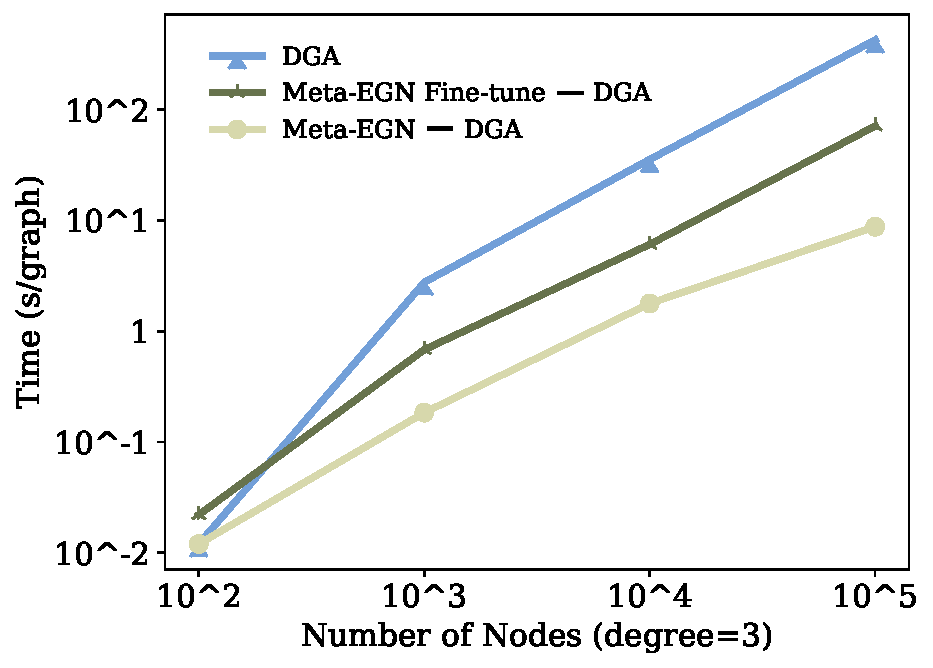
\includegraphics[width=0.32\textwidth]{iclr2023/img/exp/time_3.pdf}
         %\vspace{-0.6cm}
         %\caption{Performance on $10^3$ nodes}
         %\label{fig:mis_ga_103}
     %\end{subfigure}
     \hfill
     %\begin{subfigure}[c]{0.31\textwidth}
         %\centering
         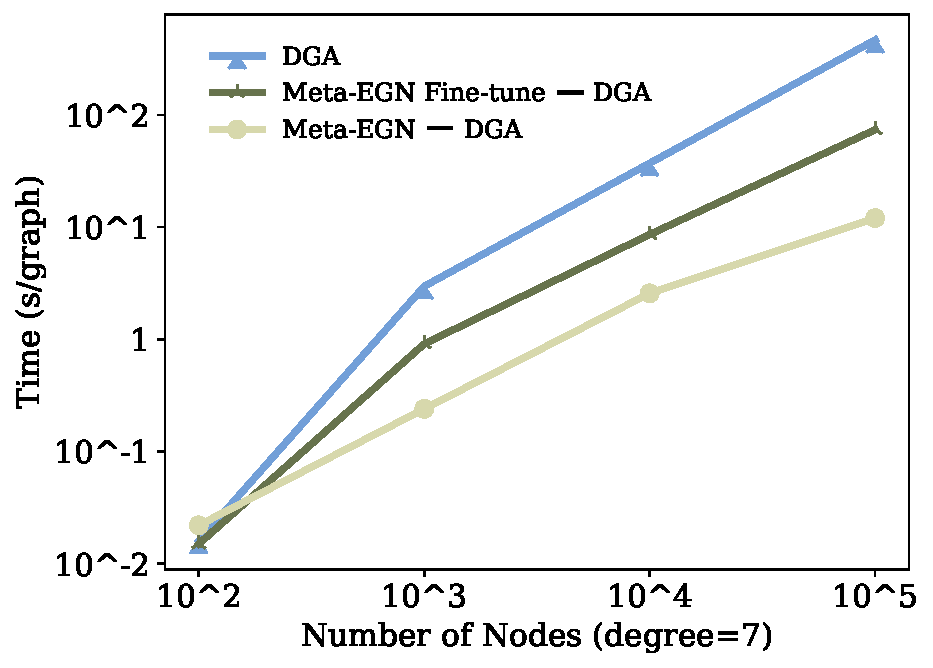
\includegraphics[width=0.32\textwidth]{iclr2023/img/exp/time_7.pdf}
         %\vspace{-0.6cm}
         %\caption{Performance on $10^4$ nodes}
        % \label{fig:mis_ga_104}
     %\end{subfigure}
     \hfill
     %\begin{subfigure}[c]{0.31\textwidth}
         %\centering
         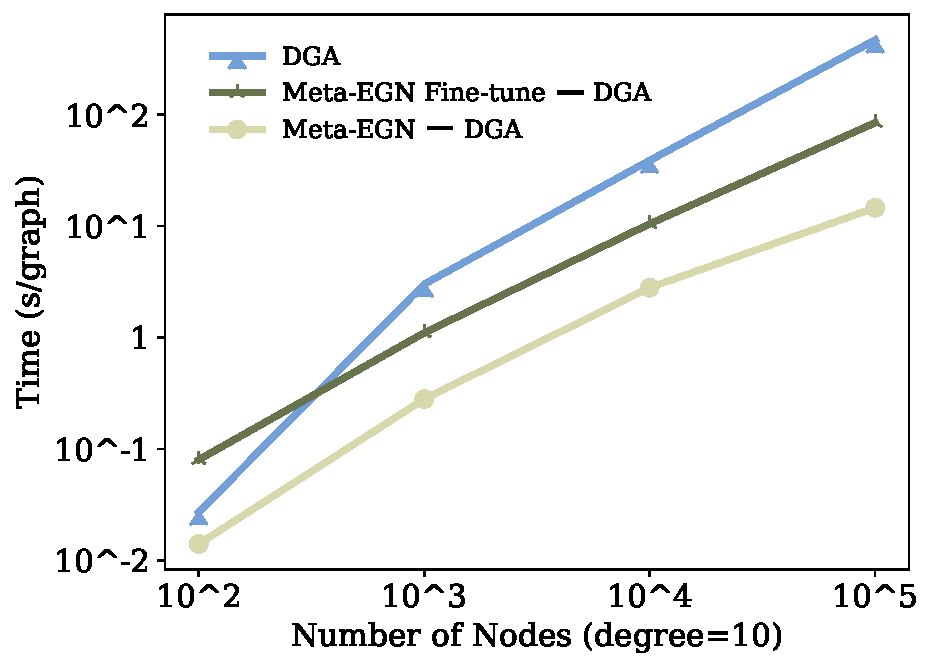
\includegraphics[width=0.32\textwidth]{iclr2023/img/exp/time_10.pdf}
         %\vspace{-0.6cm}
         %\caption{Performance on $10^5$ nodes}
         %\label{fig:mis_ga_105}
     %\end{subfigure}
     \vspace{-0.3cm}
        \caption{Time cost v.s. Graph Scales on degree $3,7,10$}
        \label{fig:mis_time_app}
\end{figure}
\subsection{How much does \proj modify DGA and RGA heuristics in the MIS}
%We provide the details that how much \proj could further modify the two heuristics DGA and RGA, as shown in Table.~\ref{tab:mis_statistics}.
We display the average approximation rate improvement and the average node number increase by Meta-EGN over DGA and RGA in Table.~\ref{tab:mis_statistics}.
\begin{table}[h]
\caption{Improvement of \proj over DGA and RGA in the MIS on RRGs, `Imp in ApR' denotes the average improvement in approximation rate, and `Imp in $\#$Node' denotes the average number of nodes that \proj could find more than the heuristics.}
\label{tab:mis_statistics}
\vspace{-0.3cm}
\resizebox{1.0\textwidth}{!}{\begin{tabular}{@{}cccc|cc|cc|cc@{}}
\toprule
 & \multirow{2}{*}{Scale$/$Degree} & \multicolumn{2}{c|}{3} & \multicolumn{2}{c|}{7} & \multicolumn{2}{c|}{10} & \multicolumn{2}{c}{20} \\ \cmidrule(l){3-10} 
 &  & Imp in ApR & Imp in $\#$Node & Imp in ApR & Imp in $\#$Node & Imp in ApR & Imp in $\#$Node & Imp in ApR & Imp in $\#$Node \\ \midrule
\multirow{3}{*}{\proj improves DGA by} & $10^3$ & 0.0043 & 1.950 & 0.0060 & 2.014 & 0.0044 & 1.254 & 0.0084 & 1.657 \\
 & $10^4$ & 0.0050 & 22.768 & 0.0062 & 20.811 & 0.0067 & 19.109 & 0.0079 & 15.588 \\
 & $10^5$ & 0.0032 & 145.718 & 0.0045 & 151.051 & 0.0051 & 145.69 & 0.0050 & 98.660 \\ \midrule
\multirow{3}{*}{\proj improves RGA by} & $10^3$ & 0.0944 & 42.986 & 0.1208 & 40.549 & 0.1292 & 36.849 & 0.1239 & 24.447 \\
 & $10^4$ & 0.0932 & 424.404 & 0.1125 & 377.628 & 0.1151 & 328.276 & 0.1173 & 231.456 \\
 & $10^5$ & 0.0871 & 3966.272 & 0.1045 & 3507.751 & 0.1083 & 3088.824 & 0.0969 & 1912.030 \\ \bottomrule 
\end{tabular}}
\end{table}

\subsection{Training the Models on Subsets of the Training Data}
We display the average approximation rates of the models that are only trained on subsets of the original training data in the max clique problem on Twitter. The training dataset is randomly sampled from the original training dataset and the testing dataset remains the same as that in Table.~\ref{tab:mc_performance}. Both methods have worse performance as the number of training instances reduces, while Meta-EGN only has a $0.7\%$ performance decrease from the full-size training dataset with 750 samples to the training subset with only $64$ instances. In contrast, EGN decreases its performance by $1.7\%$.


\begin{table}[h]
\caption{The approximation rate of the max clique problem on Twitter. Models are only trained on subsets of the dataset, `training subset' denotes the number of instances in the training data.}
\centering
\begin{tabular}{@{}cccccc@{}}
\toprule
training subset & 64          & 128         & 256         & 512         & Full (750)  \\ \midrule
EGN           & 0.909±0.122 & 0.911±0.118 & 0.914±0.118 & 0.922±0.115 & 0.926±0.113 \\
Meta-EGN      & 0.970±0.058 & 0.973±0.055 & 0.975±0.055 & 0.975±0.051 & 0.976±0.048 \\ \bottomrule
\end{tabular}
\end{table}

\subsection{Training the Models on RRGs with single Degrees in the MIS}
We train the EGN and Meta-EGN models on RRGs with only $3$ or $20$ degrees and test them on RRGs with the rest of degrees from $\{3, 7, 10, 20\}$. Models take the output of DGA as the initialization graph node feature. We show the performance of both the models without fine-tuning in Fig.~\ref{fig:train_only3_20}. When only trained on RRGs with degree $3$ (See the left two figures in Fig.~\ref{fig:train_only3_20}), both the models could not generalize well, as neither of them could outperform the initialization input of DGA. Note that Meta-EGN still achieves better performance than EGN in this case. As to the models only trained on RRGs with degree $20$ (See the right two figures in Fig.~\ref{fig:train_only3_20}), we observe that both the model have relatively good generalization ability across different degrees, yet Meta-EGN could still marginally outperform EGN in this case. We attribute this phenomenon to the fact that solving the MIS on RRGs with degree $20$ is much more complicated than those with degree $3$ and thus may contain adequate heuristics for solving RRGs with lower degrees.


\begin{figure}[h]
     \centering
         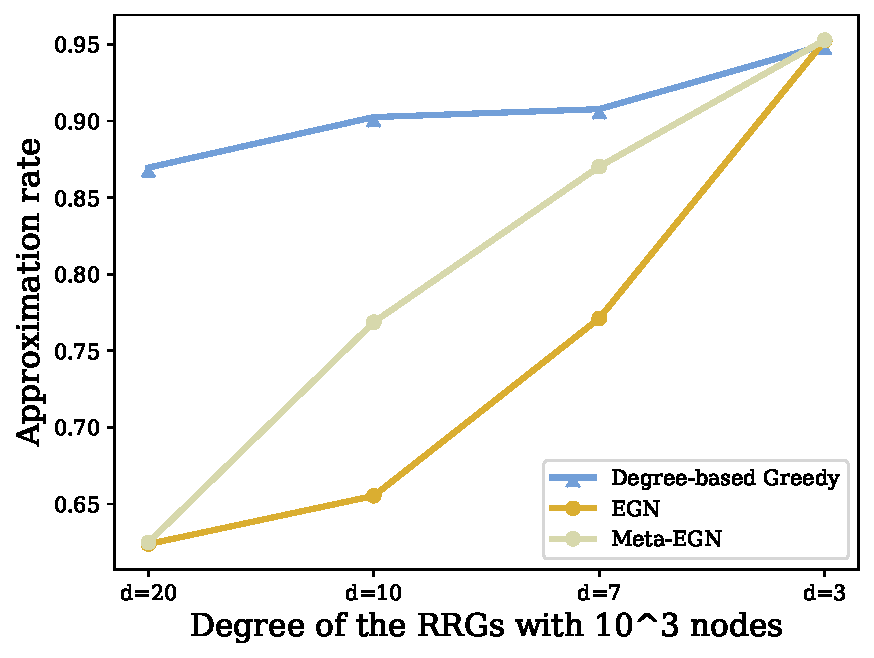
\includegraphics[width=0.23\textwidth]{iclr2023/img/app/mis_10_3_app3.pdf}
     \hfill
         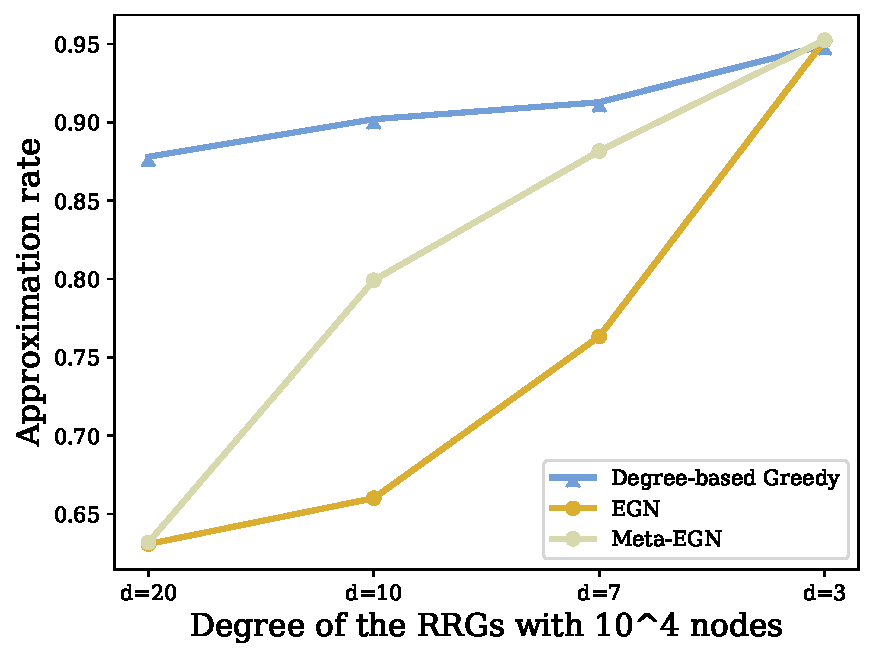
\includegraphics[width=0.23\textwidth]{iclr2023/img/app/mis_10_4_app3_.pdf}
     \hfill
         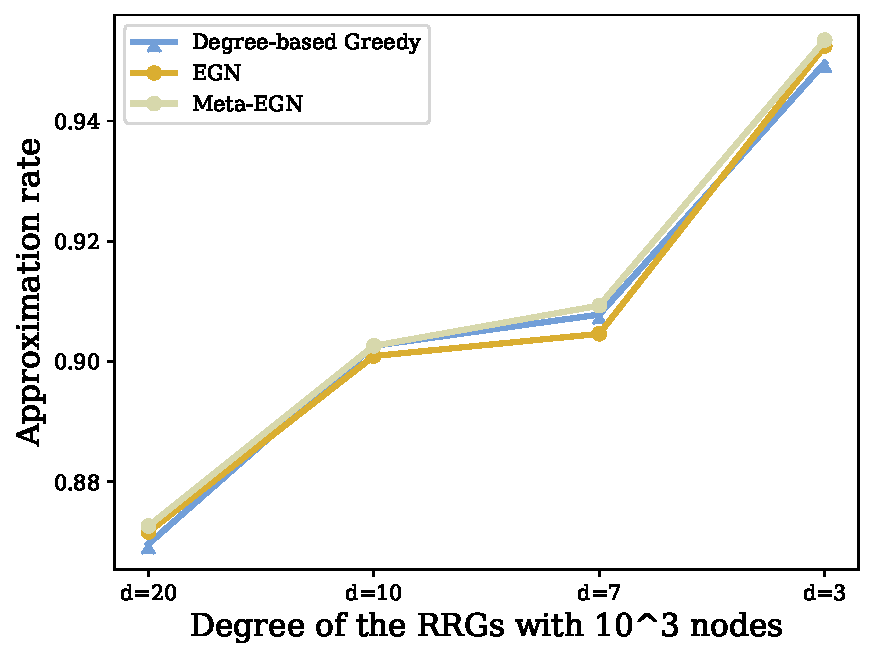
\includegraphics[width=0.23\textwidth]{iclr2023/img/app/mis_10_3_app20.pdf}
    \hfill
        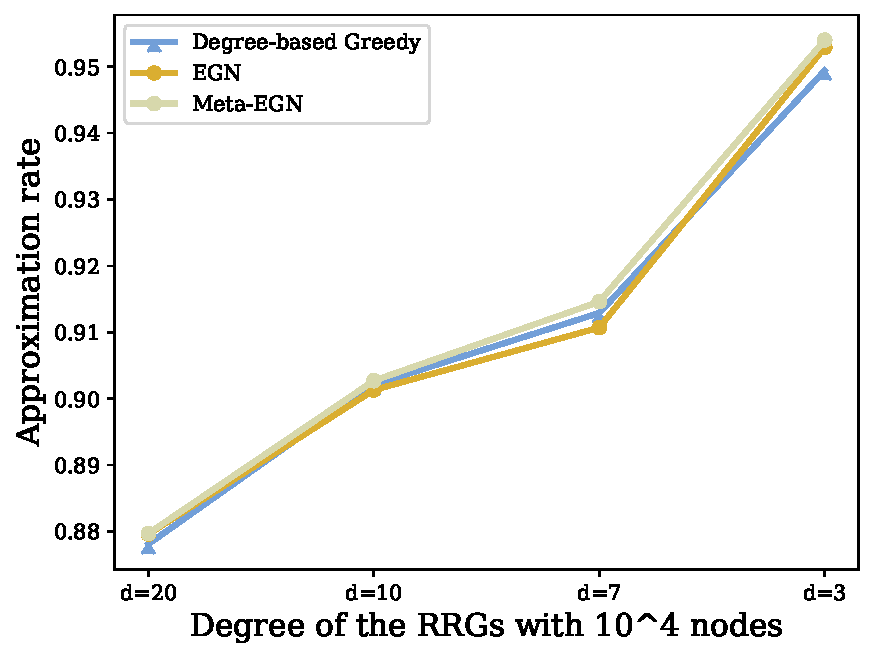
\includegraphics[width=0.23\textwidth]{iclr2023/img/app/mis_10_4_app20.pdf}
     \vspace{-0.3cm}
        \caption{The left two figures show the ApRs on RRGs with $10^3$ and $10^4$ nodes of the models trained only on RRGs with degree $3$. The right two figures show the ApRs on RRGs with $10^3$ and $10^4$ nodes of the models trained only on RRGs with degree $20$.}
        \label{fig:train_only3_20}
        \vspace{-0.3cm}
\end{figure}

\subsection{Comparison on the Training Time of the Models}
We display the wall clock training time for the two methods to converge in Table.~\ref{tab:training_time} (from start to the best epoch on validation set). We observe that Meta-EGN generally takes two to three times to converge compared with EGN, but their training time cost basically remains on the same order of magnitude.

\begin{table}[h]
\caption{The wall clock training time to convergence of EGN and Meta-EGN in different problems.}
\label{tab:training_time}
\centering
\begin{tabular}{@{}cccc|ccc|c@{}}
\toprule
\multirow{2}{*}{\begin{tabular}[c]{@{}c@{}}Dataset/Time\\ (min:second)\end{tabular}} & \multicolumn{3}{c|}{MC} & \multicolumn{3}{c|}{MVC} & MIS \\
 & Twitter & RB200 & RB500 & Twitter & RB200 & RB500 & RRGs \\ \midrule
EGN & 46:50 & 104:37 & 282:57 & 100:58 & 83:27 & 128:39 & 733:02 \\
Meta-EGN & 101:55 & 210:04 & 609:47 & 276:38 & 168:25 & 282:15 & 1088:55 \\ \bottomrule
\end{tabular}
\end{table}
\section{Supplementary Implementation Details}
\label{sec:app_experiment_details}
\subsection{Experiment Details}
All the codes run on the PyTorch platform 1.9.0~\citep{NEURIPS2019_9015} and PyTorch Geometric framework 1.7.2~\citep{Fey/Lenssen/2019}. The details of each dataset is shown in Table.~\ref{tab:dataset_details}, all of the real datasets are publicly available, and we follow the code in~\citep{toenshoff2021graph} to generate the RB model.
\begin{table}[h]
\caption{The number of instances in each dataset. `20/scale/degree' means that we generate $20$ testing instances for each different scale-degree pair. We generate RB1000, RB2000, and RB5000 only for testing.}
\vspace{-0.2cm}
\label{tab:dataset_details}
\resizebox{1.0\textwidth}{!}{\begin{tabular}{@{}cccccccccc@{}}
\toprule
Dataset & Twitter & COLLAB & IMDB & RB200 & RB500 & RB1000 & RB2000 & RB5000 & RRGs \\ \midrule
Training & 750 & 3600 & 800 & 2000 & 2000 & - & - & - & 3000 \\
Validation & 100 & 450 & 100 & 100 & 100 & - & - & - & 30 \\
Testing & 100 & 450 & 100 & 100 & 100 & 100 & 100 & 100 & 20/scale degree \\ \bottomrule
\end{tabular}}
\end{table}

To balance the training time per epoch of EGN and Meta-EGN, we define the epoch as follows: For each epoch of EGN training, the whole dataset is split into mini-batches. EGN performs standard mini-batch training along these batches and optimizes over each mini-batch. As to Meta-EGN, for each training epoch Meta-EGN only randomly samples a single batch and does the meta learning algorithm on the batch. The batch sizes of the methods are controlled the same.

\subsection{Detailed Derivation of the Loss Function Relaxation}
In this part, we display the detailed loss function relaxation of the three problems in our study (the MC, the MVC, and the MIS). The basic idea of training loss design and relaxation follow ~\citep{karalias2020erdos,wang2022unsupervised}.
In the following derivation, we use $i,j$ to represent the nodes in graphs, we use $X_i, X_j \in \{0,1\}$ to denote the discrete assignment of the binary optimization variables, and we use $\bar{X}_i, \bar{X}_j \in [0,1]$ to denote the relaxed soft assignment of the binary optimization variables.

\textbf{The maximum clique (MC):} A clique is a set of nodes $S\in V$ such that any two distinct nodes in the set are adjacent. The MC aims to find out the clique with the largest number of nodes. We could formulated the optimization objective as follows:
\begin{equation}
\centering
    \max_{X}  \sum_{1\leq i\leq n} X_i  \quad \quad \text{s.t.} \quad  (i, j) \in E\;\text{if}\;{X_i, X_j = 1} ,
\end{equation}$X_i,X_j$ denotes whether to take the node into the clique set ($X_i = 1$) or not ($X_i = 0$). By setting a proper penalty coefficient $\beta$, we could formulate the loss function relaxation as follows (the detailed derivation follows the corresponding case study in ~\cite{karalias2020erdos}).
\begin{equation}
    l_{\text{MC}}(\theta;G) \triangleq - (\beta+1)\sum_{(i,j)\in E} \bar{X}_i \bar{X}_j + \frac{\beta}{2} \sum_{i \neq j} \bar{X}_i \bar{X}_j.
\end{equation}

\textbf{The minimum vertex covering (MVC):} A vertex cover is a set of nodes $S\in V$ that any edge in the graph is connected to at least a node from the set. The MVC aims to find out the cover set with the smallest number of nodes. The optimization objective could be summarized as follows:
\begin{equation}
    \min_{X} \sum_{1 \leq i \leq n} X_i \quad \quad \text{s.t.} \quad  X_i + X_j \geq 1\;\;\text{if}\;(i,j)\in E,
\end{equation}where $X_i,X_i$ denotes whether to take the node into the cover set ($X_i = 1$) or not ($X_i=0$). We design the constraint function $g$ to represent the total number of edges that have not been covered given a set of variable assignment $X$, and thus we write $g$ as:
\begin{equation}
    g_{\text{MVC}}(X;G) \triangleq \sum_{(i,j) \in E} (1-X_i) (1-X_j).
\end{equation}
Then we relax the constraint $g$ and add it into the training objective by multiplying a proper penalty coefficient $\beta$, following the relaxation principle in~\cite{wang2022unsupervised}:
\begin{equation}
    l_{\text{MVC}}(\theta;G) \triangleq \sum_{1\leq i \leq n} \bar{X}_i +\beta \sum_{(i,j) \in E} (1-\bar{X}_i) (1-\bar{X}_j).
\end{equation}
By this, we aim to minimize the value of the loss function above in order to minimize the node number of the cover set as well as consider the covering property in the constraint.


\textbf{The maximum independent set (MIS):} An independent set is a set of nodes where any two distinct nodes in the set are not adjacent to each other. The MIS aims to find out the independent set with the largest number of nodes. We could formulate the objective of the MIS as follows:
\begin{equation}
    \max_{X} \sum_{1 \leq i \leq n} X_i \quad \quad \text{s.t.} \quad  X_iX_j = 0 \;\text{if}\; (i,j) \in E,
\end{equation}where $X_i, X_j$ denotes whether to take the node into the independent set ($X_i = 1$) or not ($X_i = 0$). We formulate the constraint $g$ as the total number of edges whose two connected nodes at the end points are both assigned into the independent set. Therefore we could write the constraint as follows:
\begin{equation}
    g_{\text{MIS}} \triangleq \sum_{(i,j) \in E} X_i X_j.
\end{equation}
We then relax the constraint $g$ into continuous space and add it into the c function with a proper penalty coefficient $\beta$, following the relaxation principle in ~\citep{wang2022unsupervised}, and thus we could write the training loss function as:
\begin{equation}
    l_{\text{MIS}}(\theta;G) \triangleq -\sum_{1 \leq i \leq n} \bar{X}_i + \beta \sum_{(i,j) \in E} \bar{X_i} \bar{X_j}.
\end{equation}
By this, we aim to minimize the value of the loss function above in order to maximize the node number of the independent set as well as consider the independent property in the constraint.

\subsection{Separated Algorithm Tables}
We separate the algorithm table of \proj into training and testing parts to make it clearer. The algorithm table is shown in Alg.~\ref{method:alg_table_train} for training and Alg.~\ref{method:alg_table_test}.

\begin{algorithm}[h]
\caption{Train \proj}
\label{method:alg_table_train}
\begin{algorithmic}[1]
\Require Training instances $\Xi=\{G_1,G_2,...,G_m\}$; Hyperparameters: $\alpha, \gamma$.
\State Randomly initialize $\theta^{(0)}$
\For{each randomly sampled mini-batch $B_j\subset \Xi$, $j=0,1,...,K-1$} \Comment{Training starts}
%\State Sample instances $G_i \sim \mathbb{P}_G$ 
%\For {$K$ steps}
%\ForAll{$G_i\in B_j$}
%\State Evaluate $\nabla_{\theta}l(\theta;G_i)$
\State For each $G_i\in B_j$, compute the adapted parameter: $\theta_i^{(j)} = \theta^{(j)} - \alpha \nabla_{\theta^{(j)}}l(\theta^{(j)};G_i)$
%\EndFor
\State Update: $\theta^{(j+1)} \gets \theta^{(j)} - \gamma \nabla_{\theta^{(j)}} \sum_{G_i \in B_j} l(\theta_i^{(j)};G_i)$
\EndFor \\
\Return $\theta\leftarrow \theta^{(K)}$
\Comment{Training ends}
\end{algorithmic}
\end{algorithm}

\begin{algorithm}[h]
\caption{Test \proj with/without Fine-tuning}
\label{method:alg_table_test}
\begin{algorithmic}[1]
\Require Testing instance $G'$; Hyperparameter: $\alpha$; Pre-trained parameter initialization $\theta$.
\State For a given testing instance $G'$: \Comment{Testing starts}
\If {fine-tuning is allowed} 
\State Fine-tune the parameters: $\theta_{G'} \gets \theta - \alpha \nabla_{\theta} l(\theta; G')$ 
\State Use Def.~\ref{def:rounding} to round the relaxed solution given by $\mathcal{A}_{\theta_{G'}} (G')$ \Comment {With fine-tuning}
%\State Rounding for discrete solution 
\Else
\State Use Def.~\ref{def:rounding} to round the relaxed solution given by $\mathcal{A}_{\theta} (G')$ \Comment {Without fine-tuning}
%\State Rounding for discrete solution
\EndIf \\
\Return the rounded solution \Comment{Testing ends}
\end{algorithmic}
\end{algorithm}





\subsection{Implementation of the heuristics}
\label{sec:greedy_implementation}
We run all of the greedy algorithms with PyThon 3.8 in this paper. A potential method to boost the time cost of these greedy algorithms is to use c++.

\textbf{Random Greedy Algorithm for MIS (RGA):} RGA takes a time to reach a solution that is linear in the problem size n. It starts from an empty independent set $S$. At each step $1 \leq t \leq n$, a node $i$ is chosen at random from the graph $G_t$ and added to the independent set. Then all the neighbors of $i$ are removed from $G_t$ to formulate a new graph $G_{t+1}$. The process iterates until $G_{t^*}$ is empty at step $t^*$, the solution is $S$.

\textbf{Degree-based Greedy Alforithm for MIS (DGA):} DGA modifies RGA by sorting the degrees of the nodes before each iteration starts, and always put the node with the smallest degree into the independent set.

\textbf{Teonshoff Greedy for MC:} ~\cite{toenshoff2021graph} convert the testing instances into its complement graph, and then run DGA to solve the MIS problem. It takes the solution to the MIS problem on the complement graph as the solution for MC on the original graph.

\textbf{Greedy for MVC:} Greedy for MVC starts from an empty covering set $S$. At each step $1 \leq t \leq n$, it first sorts the degrees of the nodes in the graph $G_t$ and always adds the node $i$ with the largest degree into the covering set $S$. Then all the edges that connect with $i$ are removed from $G_t$ to formulate a new graph $G_{t+1}$. The process stops until $G_{t^*}$ is empty at step $t^*$, the solution is $S$.

\section{Discussion on Limitations}
$\bullet$ As mentioned at the end of Sec.~\ref{sec:settings}, both EGN and Meta-EGN perform generally well in MC, which outputs the cliques that are more local in comparison with the vertex covering in MVCs that require more global assignments. The random initialization seed with one node randomly set as $1$ and the others as $0$ would potentially limit the performance of EGN and Meta-EGN in more global CO tasks.

$\bullet$ We use Meta-EGN and EGN to modify the solution of DGA and RGA in the MIS problem. In addition, there are also many other Monte Carlo (MC) algorithms (i.e. simulated annealing and parallel tempering) that could produce better results than DGA or RGA in RRGs~\citep{angelini2022cracking}. An intuitive idea is to test whether we could learn Meta-EGN to further fine-tune these more advanced MC algorithms in the MIS problem on RRGs. 

We leave the research on modifying \proj to better deal with the CO problems that require global assignments and using \proj to improve other advanced MC algorithms as a future study.




\iffalse
\begin{table}[]
\fontsize{6}{8}\selectfont
\setlength\tabcolsep{3pt}
    \begin{minipage}{1.00 \linewidth}
     \centering
     \begin{tabular}{@{}ccccccc@{}}
\toprule
                  & Twitter             & COLLAB  & IMDB    & RB test & RB 200 & RB 500 \\ \midrule
EGN               & 1.109 \hspace{-0.3mm}$\pm$\hspace{-0.3mm} 0.105(0.20) & 1.004 \hspace{-0.3mm}$\pm$\hspace{-0.3mm} 0.044 (0.04) & 1.030 \hspace{-0.3mm}$\pm$\hspace{-0.3mm} 0.170 (0.02) &     1.106 \hspace{-0.3mm}$\pm$\hspace{-0.3mm} 0.260 (0.28)    &    1.478 \hspace{-0.3mm}$\pm$\hspace{-0.3mm} 0.512 (0.31)    &    1.281 \hspace{-0.3mm}$\pm$\hspace{-0.3mm} 0.092 (0.33)    \\
EGN f-t           & 1.094 \hspace{-0.3mm}$\pm$\hspace{-0.3mm} 0.100(0.72) & 1.000 (0.13) & 1.000 (0.18) &    1.079 \hspace{-0.3mm}$\pm$\hspace{-0.3mm} 0.178 (0.75)     &    1.232 \hspace{-0.3mm}$\pm$\hspace{-0.3mm} 0.120 (0.89)    &    1.172 \hspace{-0.3mm}$\pm$\hspace{-0.3mm} 0.101 (0.90)    \\
\proj          & \textbf{1.059 \hspace{-0.3mm}$\pm$\hspace{-0.3mm} 0.070(0.20)} & 1.000 (0.04) & 1.000 (0.02) &    \textbf{1.101 \hspace{-0.3mm}$\pm$\hspace{-0.3mm} 0.267 (0.28)}     &    1.465 \hspace{-0.3mm}$\pm$\hspace{-0.3mm} 0.495 (0.31)    &    \textbf{1.267 \hspace{-0.3mm}$\pm$\hspace{-0.3mm} 0.092 (0.33)}    \\
\proj f-t      & 1.044 \hspace{-0.3mm}$\pm$\hspace{-0.3mm} 0.070(0.72) & 1.000 (0.13) & 1.000 (0.18) &    1.068 \hspace{-0.3mm}$\pm$\hspace{-0.3mm} 0.170 (0.75)     &    1.232 \hspace{-0.3mm}$\pm$\hspace{-0.3mm} 0.112 (0.89)    &    \textbf{1.150 \hspace{-0.3mm}$\pm$\hspace{-0.3mm} 0.103 (0.90)}    \\ \midrule
Greedy            &        \textbf{1.101 \hspace{-0.3mm}$\pm$\hspace{-0.3mm} 0.093 (0.12)}             &     \textbf{1.000 (0.07)}    &     \textbf{1.000 (3e-3)}    &    \textbf{1.030 \hspace{-0.3mm}$\pm$\hspace{-0.3mm} 0.118 (0.33)}     &   \textbf{1.154 \hspace{-0.3mm}$\pm$\hspace{-0.3mm} 0.124 (0.29)}     &    \textbf{1.157 \hspace{-0.3mm}$\pm$\hspace{-0.3mm} 0.089 (0.35)}    \\ \midrule
Gurobi9.5 ($\leq$0.25s) &    -      &    -     &    1.000 (0.01)     &  -       &   -     &     -   \\
Gurobi9.5 ($\leq$1.00s) &       \textbf{1.000 (0.61)}              &    1.058 \hspace{-0.3mm}$\pm$\hspace{-0.3mm} 0.557 (0.70)     &    1.000 (0.01)     &   -      &   \textbf{1.023 \hspace{-0.3mm}$\pm$\hspace{-0.3mm} 0.057 (0.95)}     &    -    \\
Gurobi9.5 ($\leq$2.00s) & 1.000 (0.61)         &    1.000 (0.72)     &    1.000 (0.01)     &     -    &  \textbf{1.009 \hspace{-0.3mm}$\pm$\hspace{-0.3mm} 0.036 (1.09)}      &    1.271 \hspace{-0.3mm}$\pm$\hspace{-0.3mm} 0.325 (11.10)    \\
Gurobi9.5 ($\leq$15.00s) &      1.000 (0.61)              &    1.000 (0.72)     &     1.000 (0.01)    &     1.210 \hspace{-0.3mm}$\pm$\hspace{-0.3mm} 1.131 (8.79)    &    1.009 \hspace{-0.3mm}$\pm$\hspace{-0.3mm} 0.036 (1.09)   &    \textbf{1.099 \hspace{-0.3mm}$\pm$\hspace{-0.3mm} 0.094 (13.34)}    \\ \bottomrule
\end{tabular}
    \vspace{-0.3cm}
     \caption{Evaluation on the minimum dominating set (MDS) problem.}
     \label{tab:mds_performance}
    \end{minipage}
\end{table}




\resizebox{1.0\textwidth}{!}{\begin{tabular}{@{}cc|ccc|ccc|ccc|ccc@{}}
\toprule
\multirow{2}{*}{Dataset} & \multirow{2}{*}{Method} & \multicolumn{3}{c|}{Fast (1)} & \multicolumn{3}{c|}{Medium (4)} & \multicolumn{3}{c|}{Accurate (8)} & \multicolumn{3}{c}{Fine-tune} \\
 &  & Approximation Rate & Gap & Rank & Approximation Rate & Gap & Rank & Approximation Rate & Gap & Rank & Approximation Rate & Gap & Rank \\ \midrule
\multirow{4}{*}{RB1000} & time/s & \multicolumn{3}{c|}{0.05} & \multicolumn{3}{c|}{0.17} & \multicolumn{3}{c|}{0.33} & \multicolumn{3}{c}{0.98} \\
 & EGN & 0.6462±0.282 & 11.48 & 2.406 & 0.8433±0.229 & 6.47 & 2.237 & 0.9099±0.205 & 4.86 & 2.025 & 0.9631±0.186 & 4.13 & 1.693 \\
 & \proj & 0.7692±0.276 & 8.57 & 1.943 & \textbf{0.9388±0.196} & \textbf{4.61} & \textbf{1.543} & \textbf{0.9408±0.205} & \textbf{4.97} & \textbf{1.581} & \textbf{0.9745±0.195} & \textbf{4.01} & \textbf{1.625} \\
 & Gurobi9.5 & \textbf{0.8851±0.197(6.11)} & \textbf{5.08} & \textbf{1.650} & 0.8851±0.197(6.18) & 5.08 & 2.218 & 0.8851±0.197(6.48) & 5.08 & 2.393 & 0.8851±0.197(7.01) & 5.08 & 2.681 \\ \midrule
\multirow{4}{*}{RB2000} & time/s & \multicolumn{3}{c|}{0.10} & \multicolumn{3}{c|}{0.29} & \multicolumn{3}{c|}{0.58} & \multicolumn{3}{c}{2.03} \\
 & EGN & 0.6793±0.290 & 12.38 & 2.408 & 0.8968±0.184 & 5.23 & 2.136 & 0.9454±0.160 & 3.81 & 2.208 & 0.9714±0.154 & 3.61 & 1.983 \\
 & \proj & 0.8077±0.114 & 8.13 & 1.991 & \textbf{0.9783±0.157} & \textbf{3.48} & \textbf{1.591} & \textbf{0.9958±0.146} & \textbf{1.28} & \textbf{1.466} & \textbf{1.0112±0.134}$^*$ & \textbf{0.55} & \textbf{1.483} \\
 & Gurobi9.5 & \textbf{0.9510±0.145(24.14)} & \textbf{3.01} & \textbf{1.600} & 0.9510±0.145(24.56) & 3.01 & 2.091 & 0.9510±0.145(25.01) & 3.01 & 2.325 & 0.9510±0.145(25.66) & 3.01 & 2.533 \\ \midrule
\multirow{4}{*}{RB5000} & time/s & \multicolumn{3}{c|}{0.33} & \multicolumn{3}{c|}{1.02} & \multicolumn{3}{c|}{2.50} & \multicolumn{3}{c}{9.66} \\
 & EGN & 0.9603±0.159 & 2.42 & 2.130 & 1.0203±0.139$^*$ & -1.26 & 2.060 & 1.0272±0.140$^*$ & -1.68 & 1.980 & 1.0475±0.188$^*$ & -2.86 & 1.970 \\
 & \proj & \textbf{1.0288±0.138}$^*$ & \textbf{-1.62} & \textbf{1.820} & \textbf{1.0684±0.233}$^*$ & \textbf{-4.02} & \textbf{1.820} & \textbf{1.0727±0.234}$^*$ & \textbf{-4.42} & \textbf{1.790} & \textbf{1.0778±0.233}$^*$ & \textbf{-4.72} & \textbf{1.710} \\
 & Gurobi9.5 & 1.0000(201.55) & 0.00 & 2.050 & 1.0000(202.36) & 0.00 & 2.120 & 1.0000(205.64) & 0.00 & 2.230 & 1.0000(214.35) & 0.00 & 2.320 \\
 & Gurobi9.5 & 1.0000(3000) & 0.00 & - & 1.0000(3000) & 0.00 & - & 1.0000(3000) & 0.00 & - & 1.0000(3000) & 0.00 & - \\ %\bottomrule
%\end{tabular}}
     %\vspace{-0.2cm}
     %\centering
     %\fontsize{6}{7}\selectfont
%\setlength\tabcolsep{1pt}
%\resizebox{1.0\textwidth}{!}{\begin{tabular}{@{}cc|ccc|ccc|ccc|ccc@{}}
%\toprule
%\multirow{2}{*}{Dataset} & \multirow{2}{*}{Method} & \multicolumn{3}{c|}{Fast (1)} & \multicolumn{3}{c|}{Medium (4)} & \multicolumn{3}{c|}{Accurate (8)} & \multicolumn{3}{c}{Fine-tune} \\
 %&  & Approximation Rate & Gap & Rank & Approximation Rate & Gap & Rank & Approximation Rate & Gap & Rank & Approximation Rate & Gap & Rank \\ 
 \midrule
\multirow{4}{*}{RB1000} & time/s & \multicolumn{3}{c|}{0.20} & \multicolumn{3}{c|}{0.72} & \multicolumn{3}{c|}{1.37} & \multicolumn{3}{c}{3.05} \\
 & EGN & 1.0161±0.0048 & 16.46 & 2.250 & 1.0135±0.0013 & 13.73 & 1.920 & 1.0138±0.0013 & 13.29 & 1.860 & 1.0138±0.0013 & 13.28 & 1.960 \\
 & \proj & 1.0145±0.0016 & 14.81 & 1.935 & \textbf{0.0131±0.0012} & \textbf{13.40} & \textbf{1.700} & \textbf{1.0125±0.0012} & \textbf{12.75} & \textbf{1.545} & \textbf{1.0124±0.0012} & \textbf{12.69} & \textbf{1.455} \\
 & Gurobi9.5 & \textbf{1.0143±0.0018(1.92)} & \textbf{14.58} & \textbf{1.835} & 1.0143±0.0018(2.58) & 14.58 & 2.380 & 1.0143±0.0018(3.08) & 14.58 & 2.595 & 1.0143±0.0018(4.96) & 14.58 & 2.585 \\ \midrule
\multirow{4}{*}{RB2000} & time/s & \multicolumn{3}{c|}{0.34} & \multicolumn{3}{c|}{1.32} & \multicolumn{3}{c|}{2.69} & \multicolumn{3}{c}{6.27} \\
 & EGN & 1.0114±0.0026 & 22.02 & 2.350 & 1.0096±0.0008 & 18.57 & 1.765 & 1.0094±0.0007 & 18.17 & 1.765 & 1.0093±0.0007 & 17.98 & 1.890 \\
 & \proj & \textbf{0.0103±0.0015} & \textbf{19.94} & \textbf{1.740} & \textbf{1.0095±0.0008} & \textbf{18.41} & \textbf{1.635} & \textbf{1.0092±0.0007} & \textbf{17.82} & \textbf{1.510} & \textbf{1.0090±0.0006} & \textbf{17.38} & \textbf{1.360} \\
 & Gurobi9.5 & 1.0104±0.0010(5.63) & 20.18 & 2.910 & 1.0104±0.0010(6.65) & 20.18 & 2.600 & 1.0104±0.0010(8.04) & 20.18 & 2.725 & 1.0104±0.0010(13.24) & 20.18 & 2.750 \\ \midrule
\multirow{4}{*}{RB5000} & time/s & \multicolumn{3}{c|}{1.01} & \multicolumn{3}{c|}{3.99} & \multicolumn{3}{c|}{7.95} & \multicolumn{3}{c}{18.41} \\
 & EGN & 1.0071±0.0014 & 34.19 & 2.170 & 1.0064±0.0004 & 30.83 & 1.985 & 1.0062±0.0004 & 29.87 & 1.865 & 1.0062±0.0004 & 29.68 & 1.960 \\
 & \proj & \textbf{1.0067±0.0005} & \textbf{32.51} & \textbf{2.045} & \textbf{1.0062±0.0005} & \textbf{29.96} & \textbf{1.600} & \textbf{1.0061±0.0004} & \textbf{29.44} & \textbf{1.555} & \textbf{1.0060±0.0003} & \textbf{29.15} & \textbf{1.470} \\
 & Gurobi9.5 & 1.0066±0.0006(24.60) & 31.88 & 1.785 & 1.0066±0.0006(28.72) & 31.88 & 2.415 & 1.0066±0.0006(32.16) & 31.88 & 2.580 & 1.0066±0.0006(42.62) & 31.88 & 2.570 \\ \bottomrule
\end{tabular}}
\fi


